\documentclass{nle}

% \documentclass[sigconf]{acmart}
% \settopmatter{printacmref=false} % Removes citation information below abstract
% \renewcommand\footnotetextcopyrightpermission[1]{} % removes footnote with conference information in first column
% \pagestyle{plain} % removes running headers
% \setcopyright{none}

\usepackage{booktabs} % For formal tables
\usepackage[ruled]{algorithm2e} % For algorithms
\renewcommand{\algorithmcfname}{ALGORITHM}
\SetAlFnt{\small}
\SetAlCapFnt{\small}
\SetAlCapNameFnt{\small}
\SetAlCapHSkip{0pt}
\IncMargin{-\parindent}

\usepackage[utf8]{inputenc}
\usepackage{graphicx}
\usepackage{mathtools}
\usepackage{amsfonts}
\usepackage{multirow}

\DeclareMathOperator*{\argmax}{arg\,max\,}
\renewcommand{\arraystretch}{1.2}

\begin{document}

\title{Web data extraction through named entity labeling}

% \author{
%   João Mateus de Freitas Veneroso
%   % Universidade Federal de Minas Gerais
% }
\author[João Mateus de Freitas Veneroso and Berthier Ribeiro-Neto]
       {João Mateus de Freitas Veneroso \and
        Berthier Ribeiro-Neto\\
	Universidade Federal de Minas Gerais\\
	Belo Horizonte - MG, Brazil}

% \affiliation{%
%   \institution{Universidade Federal de Minas Gerais}
%   \streetaddress{Av. Pres. Antônio Carlos, 6627 - Pampulha}
%   \city{Belo Horizonte}
%   \state{MG}
%   \postcode{31270-901}
%   \country{Brazil}}
% \email{jmfveneroso@gmail.com}
% 
% \author{Berthier Ribeiro-Neto}
% \affiliation{%
%   \institution{Universidade Federal de Minas Gerais}
%   \streetaddress{Av. Pres. Antônio Carlos, 6627 - Pampulha}
%   \city{Belo Horizonte}
%   \state{MG}
%   \postcode{31270-901}
%   \country{Brazil}}
% \email{berthier@dcc.ufmg.br}
% \email{berthier@google.com}

\begin{abstract}

Web data extraction methods often rely on hand-coded rules to 
identify and extract data from web pages. These methods are usually
suited for extracting information from pages with repeating templates within
the same website, however they perform poorly on extraction 
tasks across different websites. Alternatively, statistical and 
machine-learning-based sequence labeling methods provide a more flexible 
approach to Web data extraction. Many times, HTML pages are very different 
from plain text, because sentences are too short to provide adequate 
context for conventional Named Entity Recognition methods to work 
properly. Also, the HTML structure may encode information that is not 
replicated in the text. Nonetheless, these limitations can be overcome by
adequate feature engineering, the use of pretrained word 
embeddings and neural character representations. In this article, we 
evaluate the performance of different methods of named entity recognition 
on the task of Web data extraction. In particular, we introduce a novel 
dataset~\footnote{The dataset and all models discussed in this article are available in: https://github.com/jmfveneroso/ner.} 
consisting of faculty listings from university web pages across
the world in multiple languages and test the NER models on the task of 
extracting researcher names from these listings. We found that a 
neural network architecture that combines a bidirectional LSTM with
a Conditional Random Fields output layer and LSTM-based character 
representations outperforms other methods on the researcher name 
extraction task, achieving an F1-score of 0.8867 with no feature engineering. 
With the addition of hand crafted features, the F1-score can be slightly 
improved to 0.8995.

\end{abstract}

\maketitle

% \textbf{Declarations of interest: none} \\
% \\
% \\
João Mateus de Freitas Veneroso \\
Mailing address: Universidade Federal de Minas Gerais, Departmento de Ciência da Computação, sala 4304\\
Av. Pres. Antônio Carlos, 6627 - Pampulha, Belo Horizonte - MG, 31270-901 \\
Tel: +55 (31) 99436-0909 \\
Email: jmfveneroso@gmail.com \\

Berthier Ribeiro-Neto \\
Mailing address: Universidade Federal de Minas Gerais, Departmento de Ciência da Computação, sala 4321\\
Av. Pres. Antônio Carlos, 6627 - Pampulha, Belo Horizonte - MG, 31270-901 \\
Tel: +55 (31) 99313-0961 \\
Email: berthier@dcc.ufmg.br \\

% \keywords{Named entity recognition, information extraction, web data extraction}

\section{Introduction}

Web data extraction (WDE) is the task of automatically extracting structured 
information from unstructured or semi-structured Web documents. The input 
usually consists of Web documents containing a number of predetermined entities 
organized in a similar manner. The web data extraction task consists of 
identifying these entities and organizing them according to a template. 

HTML documents most often lie in between the structured/unstructured 
data paradigm. DOM hierarchy, element disposition, CSS classes, and other 
features related to the document structure and indirectly associated with the 
data itself can be valuable information on the task of identifying
entities. Yet, we cannot expect these features to be completely constrained 
by an underlying pattern. Organization patterns tend to follow some guidelines 
but they are in no way subject to strict rules. That is why classical web data 
extraction systems such as automatic wrapper generators 
\cite{Kushmerick2000,Hsu1998,Muslea1999}
do not translate very well across different websites. 

Most existing Web data extraction methods are tailored to extract data 
from a single Web page, producing different compromises between efficacy and 
degree of human supervision. Some unsupervised approaches proposed to tackle 
the problem of data extraction for whole application domains 
\cite{Zhu2005,Zhu2006,Abdessalem2010,Furche2012,Furche2012a}. Usually, 
unsupervised WDE methods work in two stages. In the record segmentation stage,
WDE systems seek to cluster visually and structurally similar Web page regions 
and identify repeating data records with heuristics and 
hand-coded rules. In the attribute labeling stage, WDE systems seek to identify 
the correct attributes on data records, many times resorting to regular expressions 
or gazetteer matching strategies. The outcome of each of these stages can aid one 
another. The inner patterns of data records can help in identifying attributes of other 
data records. Also, by properly identifying data record attributes, it becomes 
easier to determine boundaries and perform record segmentation.

While unsupervised approaches can be sometimes adequate to extract information from 
Web pages with similar templates, they usually fail on cross-website data extraction 
tasks. Also, more sophisticated approaches may be needed when we are not dealing
with easily distinguishable attributes such as prices and dates. In this regard, 
machine-learning-based sequence labeling methods can provide a more flexible 
approach that works regardless of website structure.

In recent years, we saw an amazing progress in the field of Natural Language Processing, 
particularly with the introduction of deep recurrent neural network architectures
for sequence labeling. However, despite Web data extraction being a closely 
related field, there is a lack of extraction tools that make use of these recent 
advancements. The attribute labeling stage in Web data extraction systems
is essentially a Named Entity Recognition (NER) problem, the problem of 
detecting named entities in the text and classifying them into predetermined 
categories such as person names, locations, dates or organizations. 

In many cases, such as when we are extracting researcher names from faculty listings,
detecting named entities is sufficient to solve the data extraction task. However, when we are
dealing with multi-attribute data records or complex relationships, we may need to 
perform additional steps. Nevertheless, even in the latter cases, flexible NER methods 
are still desirable because, while many WDE algorithms can effectively exploit the 
semi-structured nature of Web documents, too much reliance on structural Web page 
features often produce poor generalizations on cross website extraction. Also, 
data records may enclose plain text with relevant named entities. 

In this paper, we investigate methods of named entity recognition for Web data extraction.
Recently proposed neural architectures have achieved exciting results 
on the NER task in plain text while requiring almost 
no feature engineering or access to gazetteers \cite{Huang2015,Lample2016,Ma2016}. 
NER on HTML poses a slightly different type of challenge. Named entities may occur inside 
tables, lists, or other types of visual elements that provide little to no textual 
information that could give hints about the semantic category of a word. Still, even 
with this limitation, we show that it is possible to obtain very good results with a 
relatively small training set.

By reliably detecting named entities on HTML, we can improve the performance of existing WDE 
approaches or even construct an end-to-end neural network architecture to solve domain 
wide data extraction with considerable flexibility. To test different NER approaches to
Web data extraction, we explored the task of researcher name extraction from university 
faculty listings across the world, introducing a novel NER dataset.

Reliable researcher affiliation information is often missing from public researcher 
databases (especially in departments other than Computer Science). Also, the display of 
faculty information varies significantly between different university websites, so 
this task can provide a good measure of the expected performance and data need of
NER methods on other Web data extraction tasks. 


\section{Related Work}

In the last 20 years, the astonishing growth of public information in the Web has 
led to the development of a number of different approaches to the problem of Web 
data extraction. Traditionally, the task was solved by designing special purpose
programs called wrappers to recognize relevant data and store records in a structured
format. These early tools varied wildly relative to their degree of automation. 

It was readily perceived that manual wrapper generation was a rather tedious and
error prone process, unsuited for large scale operations. Wrappers tend to
break frequently because they rely heavily on Web page features that can change 
often. So, in the late nineties, several authors advocated for wrapper induction, a technique 
that consists of automatically constructing wrappers from a small set of examples by 
identifying delimiters or context tokens that single out the desired attributes. 
Some remarkable wrapper induction methods are WIEN \cite{Kushmerick2000}, Soft 
Mealy \cite{Hsu1998} and STALKER \cite{Muslea1999}.

Despite being better than constructing wrappers manually, wrapper induction methods 
still suffered from a lack of expressive power and flexibility. These methods had 
trouble handling records with missing attributes or unusual structures because
patterns could only be identified if they happened at least once in the examples.

Other approaches such as NoDoSE \cite{Adelberg1998} and Debye \cite{Laender2002a} 
brought greater flexibility to wrapper induction methods by requiring a greater level 
of human interaction through graphical user interfaces. Web data extraction techniques often 
require some sort of assistance from human experts to boost accuracy. One of the main challenges 
in the field lies in determining an adequate trade-off between the degree of automation and 
the precision and recall of the data extraction tool.

To automate the task of Web data extraction completely some approaches,
such as Road Runner \cite{Crescenzi2001}, removed entirely the need for data examples.
Road Runner parses documents belonging to a same class (e.g. books on Amazon) and 
generates wrappers based on their similarities and differences, yielding comparable results 
to those obtained by wrapper induction methods. However, like previous approaches, it was 
unsuited for cross site extraction tasks because the learned rules were not general enough.

NLP based approaches aimed at extracting more general rules that could possibly
be employed over multiple websites. RAPIER \cite{Califf1999} is a method of rule
extraction that uses information such as part-of-speech tags and semantic classes from
a lexicon to derive patterns from a set of training examples. This approach is more
flexible than the wrapper induction methods, however it achieves much lower rates of 
recall and precision.

In 2002, a survey by Laender et al. \shortcite{Laender2002} made a thorough classification of the
early approaches with a taxonomy based on their main technology, being them: languages for
wrapper development, HTML-aware tools, NLP-based tools, Wrapper Induction Tools,
Modeling-based tools and Ontology-based tools. Some noteworthy examples from this era
are: 

\begin{itemize}
\item TSIMMIS \cite{Hammer1997} and WebOQL \cite{Arocena1999}, which are special purpose 
languages for building wrappers.

\item Road Runner \cite{Crescenzi2001}, XWRAP \cite{Liu2000} and W4F \cite{Sahuguet1999}, 
which are HTML-aware tools that infer meaningful patterns from the HTML structure.

\item RAPIER \cite{Califf1999}, SRV \cite{Freitag1998}, WHISK \cite{Soderland1999}, which 
are NLP-based tools.

\item WIEN \cite{Kushmerick2000}, Soft Mealy \cite{Hsu1998} and STALKER \cite{Muslea1999} which 
are wrapper induction methods.

\item NoDoSE \cite{Adelberg1998} and Debye \cite{Laender2002a}, which are semi supervised modeling
based tools that require some interaction with the user by means of a graphical
user interface.
\end{itemize}

In 2006, Chang et al. \shortcite{Chang2006} complemented the previous surveys with semi-supervised 
technologies such as Thresher \cite{Hogue2005}, IEPAD \cite{Chang2001} and 
OLERA \cite{Chang2004}. They differed from supervised 
and unsupervised methods because they either needed only a rough description of
data from users for extraction rule generation or some level of post processing
that needed user attention. The survey also mentioned newer unsupervised methods
such as DeLa \cite{Wang2003}, Exalg \cite{Arasu2003} and Depta \cite{Zhai2005}.

Most of the early information extraction systems were rule-based with either 
manual rule description or automatic rule learning from examples, thus they
suffered from a lack of flexibility when dealing with noisy and unstructured data.
Huge progress in the field of statistical learning led to the development of
statistical models that tried to solve this problem.

In 2008, Sarawagi \shortcite{Sarawagi2008} produced a survey that classified wrappers into
rule-based methods, statistical methods and hybrid models, bringing together 
the fields of named entity recognition, relationship extraction and information extraction. 
The rule based methods encompass most of the 
previous models. The statistical methods convert the extraction task into a token labeling 
task, identifying the target entities through the assignment of labels as in a typical 
Named Entity Recognition task. Traditionally, Hidden Markov Models \cite{Leek1997,Freitag1999}, 
Linear Chain Conditional Random Fields \cite{Lafferty2001}, and Maximum Entropy Taggers 
\cite{McCallum2000} have been the usual choice for linear sequence tagging models.
More recently, with the advancement of Natural Language Processing and Deep Learning, 
neural models outperformed previous NER methods for plain text. Huang et. al. \shortcite{Huang2015} introduced the 
bidirectional Long Short-Term Memory (LSTM) model with a Conditional Random Field (CRF) output layer
for NER. Ma and Hovy \shortcite{Ma2016} incorporated Convolutional Neural Network based character representations 
on top of the architecture. And Lample et. al. \shortcite{Lample2016} introduced
LSTM based character representations. 

Surveys by Ferrara et al. \shortcite{Ferrara2014}, Schulz et al. \shortcite{Schulz2016} and 
Varlamov et al. \shortcite{Varlamov2016} updated the previous surveys on information 
extraction methods with some interesting innovations. 
Some examples are: the Visual Box Model \cite{Krupl2005}, a data extraction system that produces 
a visualization of the Web page to exploit visual cues to identify data presented in a tabular form;
automatic wrapper adaptation \cite{Ferrara2011}, a technique that tries to reduce the cost of 
wrapper maintenance by measuring the similarity of HTML trees and adapting
wrappers to the new page structure; AutoRM \cite{Shi2015}, a method to mine
records from a single Web page by identifying similar data regions through DOM
tree analysis; Knowledge Vault \cite{Dong2014}, a method that combines different 
extraction approaches to feed a probabilistic knowledge base.

Most data extraction systems focus on extracting information from single websites
and are therefore unsuited for cross website extraction tasks. Even unsupervised
approaches that are domain independent, such as RoadRunner \cite{Crescenzi2001} 
and EXALG \cite{Arasu2003} only work well for extracting data from pages generated 
from a same template. 

A statistical approach to unsupervised domain 
independent Web data extraction was described by Zhu et al \shortcite{Zhu2005}. The 2D CRF 
model takes a Web page segmented into data blocks and employs a two dimensional conditional 
random field model to perform attribute labeling. The model was further improved
\cite{Zhu2006} to model record segmentation and attribute labeling as a joint task.
Some of the limitations of early unsupervised methods 
were also tackled by ObjectRunner \cite{Abdessalem2010} and AMBER \cite{Furche2012}. 
These methods work by annotating Web pages automatically with regular expressions, gazetteers and 
knowledge bases. They can rectify low quality annotations and even improve the annotators
by exploring regular structures in the DOM during the record segmentation phase.

Web data extraction methods have undoubtedly improved extraordinarily, but
as pointed by Schulz et al. \shortcite{Schulz2016}, it is difficult to compare the results 
achieved by competing tools, and many seem to rely excessively on heuristic methods.
In that regard, the recent advancements in sequence taggers may provide more robust and
flexible extraction tools.

\section{Named Entity Recognition Models}

Many Web data extraction systems rely on hand crafted rules or gazetteers to perform
attribute annotation. Machine learning approaches to NER can improve annotations of 
more complex entities and even perform entity detection without any feature
engineering. We explored many methods of Named Entity Recognition
in the context of a Web data extraction task. First, we discuss two traditional 
approaches: Hidden Markov Models, and Linear Chain Conditional Random Fields. Then,
we discuss neural network architectures.

\subsection{Hidden Markov Models}

A Markov Model is a stochastic model that computes the most probable sequence of states 
given a limited set of observable states $ S = \{s_1, s_2, ..., s_n \} $.
The Hidden Markov Model (HMM) differs from the Markov Model in that it
does not observe the states directly, but rather a probabilistic function of those 
states. For example in NER, the words are observed, however the Named Entity labels
associated with these words are not. Formally, we want to compute the most probable
sequence of labels $ Y = \{y_1, y_2, ..., y_n\} $ for a sequence of observed tokens
$ X = \{x_1, x_2, ..., x_n\} $.

\begin{equation}
Y^* = \argmax_{Y} P(Y|X)
\end{equation}

With Bayes theorem, we can write $ P(Y|X) $ as:

\begin{equation}
P(Y|X) = \frac{P(X|Y) P(Y)}{P(X)}
\end{equation}

Since $ P(X) $ is the same for all label sequences $ Y $, we can simply maximize
the probability $ P(X|Y) P(Y) $.

A HMM makes two assumptions. First, the probability of being in a given state depends 
only on a fixed number of previous states. That is:

\begin{equation}
P(y_i|y_{i-1}x_{i-1}, y_{i-2}x_{i-2}, ..., y_1x_1) = P(y_i|y_{i-1}, y_{i-2},..., y_{i-k})
\end{equation}

In fact, we can get much better results on the NER task by looking at trigrams
or quadrigrams ($ k = 2 $ or $ k = 3 $) instead of bigrams as with a regular HMM. 
Some label assignments are highly improbable, such as single token named entities 
separated by a common word. These kinds of patterns can be perceived by a higher order HMM.
Second, the probability of a word depends only on its assigned label. That is:

\begin{equation}
P(x_i|y_{i-1}x_{i-1}, ..., y_1x_1) = P(x_i|y_i)
\end{equation}

With these assumptions, 
the probability $ P(Y|X) $ can be approximated by the expression:

\begin{equation}
P(Y|X) \propto \prod_{i=k+1}^{n} P(y_i|y_{i-1}, y_{i-2}, ..., y_{i-k}) P(x_i|y_i)
\end{equation}

All relevant probabilities can be estimated through maximum likelihood estimation from the relative
frequencies of labels and features in the corpus. The best sequence of labels can be computed 
with a variable state Viterbi approach \cite{Li2000}. However, as we increase $ k $, this computation 
becomes exponentially more expensive. The beam-search strategy may be employed for a faster 
search, but we found that for $ k \leq 4 $, the Viterbi algorithm is still viable.

HMM based taggers have been successfully applied in many NLP and WDE tasks 
\cite{Rabiner1990,Leek1997,Freitag2000}. They are incredibly fast to train and also they are very 
interpretable, making them a good choice for a first approximation. However, these models 
are highly dependent on the right selection of features, what may outweigh the benefit of a 
small training cost.

\subsubsection{Self training} \label{sssec:self_training}

In the task of NER on HTML, there are useful features related to the HTML
structure that can help in identifying named entities. On a given website, named
entities tend to occur inside the same HTML tags. The HTML tag feature or other
HTML features could easily be incorporated in the HMM. However, these 
features are only useful inside a single website and they cannot be generalized, 
because different websites use distinct HTML templates. 
Therefore, we propose a self training strategy to obtain probabilities for
these HTML features. It is implemented like this:

\begin{itemize}
\item Train the HMM without any HTML features.
\item Compute labels for a website with the trained HMM.
\item Use the computed labels as a proxy for the actual labels in the 
website and estimate HTML feature frequencies for this website alone.
\item Recompute the labels now using the HTML feature probabilities.
\end{itemize}

In theory, this strategy could be used with any sequence tagger, however
retraining a classifier with new features can become prohibitively expensive.
This strategy is only possible because the computation of HTML feature
frequencies can be performed very quickly. This adds very little overhead 
to the original HMM and improves precision and recall by a considerable 
margin.

\subsection{Linear Chain Conditional Random Fields}

A Linear Chain Conditional Random Field (CRF) is the discriminative analog to the HMM,
it was first introduced by Lafferty \shortcite{Lafferty2001}. It is a distribution $ P(Y|X) $ that takes the form:

\begin{equation}
P(Y|X) = \frac{1}{Z(x)} \prod_{t=1}^{T} exp \left( \sum_{k=1}^{K} \theta_k f_k(y_{t-1}, y_t, X) \right)
\end{equation}
\\

where $ \theta $ is the parameter vector that we are going to learn, $ f_k(y_{t-1}, y_{t}, X) $ 
are feature functions over the current timestep $ t_y $, the previous timestep $ y_{t-1}$, 
and the observation vector $ X $. And the partition function $ Z(x) $, takes the form:

\begin{equation}
Z(x) = \sum_{Y} \prod_{t=1}^{T} exp \left( \sum_{k=1}^{K} \theta_k f_k(y_{t-1}, y_t, x) \right)
\end{equation}
\\

which is a sum over all possible label assignments $ Y $. The partition function can be efficiently
and exactly calculated with the sum-product algorithm. Parameter estimation is usually done through 
negative log likelihood minimization. The function can be optimized with techniques suitable for other 
maximum entropy models such as L-BFGS \cite{Liu1989}. The most likely label sequences can be decoded 
with the Viterbi algorithm, as was the case for HMMs.

CRFs are more general than HMMs because the transitions from $ y_{t-1} $ to $ y_{t} $ can depend 
on the whole vector of observations $ X $. This flexibility of feature functions allows for a wide range of
possibilities. Recently, CRFs have been successfully employed as the output layer in complex neural 
architectures bringing improvements over models that compute labels independently.

\subsection{Neural Network Architectures}

\begin{figure}
  \centering
  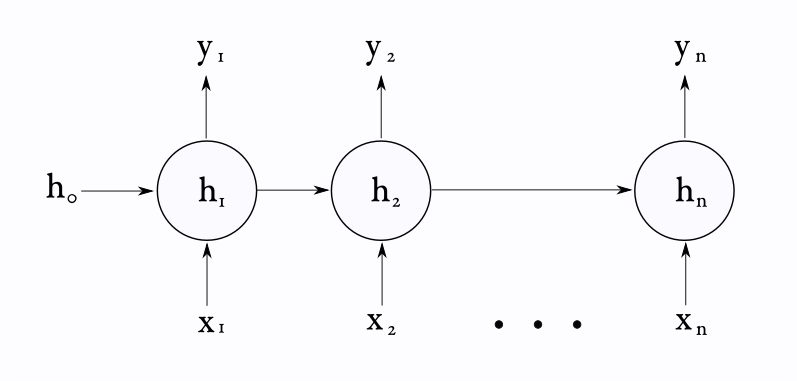
\includegraphics[width=0.75\textwidth]{pics/rnn_network}
  \caption{RNN for NER}
  \label{fig:rnn_network}
\end{figure}

Recurrent neural networks (RNN) have been successfully employed on numerous NLP tasks such as
language modelling, POS tagging, speech recognition and NER. Different from feed-forward 
neural networks, RNNs can retain information in their internal state, making them more 
suitable for processing sequences, and consequently for solving text related tasks. 
Figure~\ref{fig:rnn_network} describes an RNN for sequence labeling unrolled through multiple 
timesteps. At each timestep, the neural network computes a hidden state $ h_t $ using an input 
vector $ x_t $ and the previous hidden state $ h_{t-1} $, that retains information from past 
iterations. Finally, the RNN produces an output vector $ y_t $ representing the label for that 
timestep. A common definition for an RNN cell is given by the equations:

\begin{flalign*}
h_t &= tanh(W_x x_t + W_h h_{t-1}) &\\
y_t &= softmax(W_y h_t) &
\end{flalign*}

Where $ W_x $, $ W_h $ and $ W_y $ are weight matrices that can be trained with the 
Backpropagation Through Time (BPTT) algorithm. Theoretically, RNNs are capable of learning
and retaining long term dependencies through their internal state $ h_t $. However, in practice,
it becomes difficult due to the vanishing gradient problem. Long short term memory networks (LSTM) were 
introduced by Hochreiter and Schmidhuber \shortcite{Hochreiter1997} with this problem in mind and 
have been popularized since then. 

LSTMs incorporate a memory cell $ c $ in the RNN definition and three gates to control 
the flow of information that comes in and out of the memory cell.
The input gate $ \Gamma_{i} $ controls the amount of new information that will flow into the memory cell,
the forget gate $ \Gamma_{f} $ controls the amount of previous information that will be retained in the memory
cell, and the output gate $ \Gamma_{o} $ controls the amount of information stored in the memory cell that
will be used to compute the output activation of the LSTM unit. 
LSTM cell implementations vary slightly in the literature, a visual description of 
our LSTM cell is also provided in Figure~\ref{fig:lstm_cell}.

\begin{figure}[h]
  \centering
  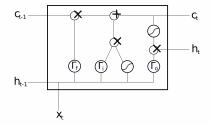
\includegraphics[width=0.75\textwidth]{pics/lstm_cell}
  \caption{LSTM Cell}
  \label{fig:lstm_cell}
\end{figure}

The equations for the LSTM cell are:

\begin{flalign*}
\Gamma_{i} &= \sigma(W_i \cdot [x_t,h_{t-1}] + b_i) &\\
\Gamma_{f} &= \sigma(W_f \cdot [x_t,h_{t-1}] + b_f) &\\ 
\Gamma_{o} &= \sigma(W_o \cdot [x_{t},h_{t-1}] + b_o) &\\
c_t        &= \Gamma_{f} \ast c_{t-1} + \Gamma_{i} \ast tanh(W_c \cdot [x_{t},h_{t-1}] + b_c) &\\
h_t        &= \Gamma_{o} \ast tanh(c_t) &
\end{flalign*}

Where $ \sigma $ is the logistic sigmoid function. $ \Gamma_i $, $ \Gamma_f $, and $ \Gamma_o $ are the input,
forget and output gates, respectively, and $ W_i $, $ W_f $, $ W_o $ are the weight 
matrices corresponding to each gate. $ c_{t} $ is the cell 
state at time $ t $ and $ h_{t} $ is the hidden state at time $ t $. 
The vector $ [x_{t},h_{t-1}] $ is formed by concatenating the current input vector 
$ x_{t} $ and the hidden vector from a previous timestep $ h_{t-1} $. Finally,
$ A \ast B $ represents the element-wise multiplication of matrices $ A $ and $ B $
and $ A \cdot B $ represents the dot product of $ A $ and $ B $.

This implementation differs from the LSTM cell described in Huang et al. \shortcite{Huang2015}
in that the gates $ \Gamma_i $ and $ \Gamma_f $ do not receive inputs from the previous 
cell state $ c_{t-1} $ and the output gate does not receive inputs from the current cell 
state $ c_{t} $. This variation produces little difference in terms of model accuracy on
the performed task, but it reduces model complexity.

\subsubsection{BI-LSTM-CRF}
\label{sssec:lstm_crf}

On named entity recognition tasks, both past and future words are important 
to attribute a label at time $ t $, however a regular LSTM network only takes 
past states into consideration. A bidirectional LSTM solves this problem by stacking 
two regular LSTMs, and feeding them with observations in opposite directions. The first LSTM 
receives forward states and the second LSTM receives backward states. The hidden states from both 
networks can then be concatenated at each timestep to produce output labels. With this 
architecture, LSTM cells may use information from past and future timesteps to decide 
the label at time $ t $.

Huang et al. \shortcite{Huang2015} proposed a bidirectional LSTM with a CRF layer (BI-LSTM-CRF) on 
the output to tackle the sequence tagging problem. The main benefit of adding a CRF layer 
in the neural sequence model is that the labels are jointly decoded for a whole sentence 
instead of being predicted individually. Another possibility would be to use a beam search
decoder to find an optimal sequence of labels. Predicted tags should be highly correlated 
in a named entity recognition task, so it is desirable to predict sequences conjointly.
The BI-LSTM-CRF is described in Figure~\ref{fig:bi_lstm_crf}.

\begin{figure}[h]
  \centering
  \includegraphics[width=0.75\textwidth]{pics/bi_lstm_crf}
  \caption{Bidirectional LSTM-CRF}
  \label{fig:bi_lstm_crf}
\end{figure}

This architecture achieved an F1 score of 90.10 on the English data from the CoNLL-2003 
NER shared task \cite{Sang2003}, in contrast to 85.17 for a bidirectional LSTM without 
a CRF layer. 
In our experiments, the LSTM-CRF architecture uses a bidirectional LSTM with 100 
hidden states, no peepholes and input and output dropout layers with a dropout
rate of 0.5. The dropout layers have proven to be very important to prevent overfitting 
and allow better generalization.

\subsubsection{CNN character representations}
\label{sssec:lstm_crf_cnn}

Ma and Hovy \shortcite{Ma2016} proposed to add a convolutional neural network (CNN) layer 
on top of a bidirectional LSTM-CRF to encode character-level information. The CNN
layer is described visually in Figure \ref{fig:cnn}.

\begin{figure}[h]
  \centering
	  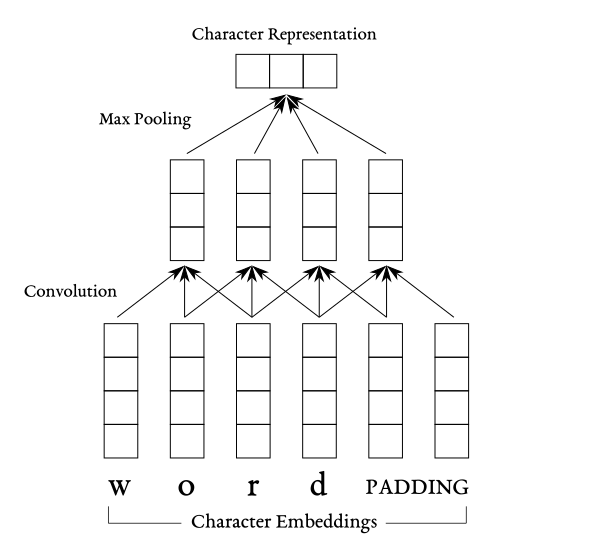
\includegraphics[width=0.75\textwidth]{pics/cnn}
  \caption{CNN based character representations}
  \label{fig:cnn}
\end{figure}

The convolutional neural network receives character embeddings as inputs. The character 
representations generated by the CNN are combined with word level representations 
and fed to the BI-LSTM-CRF in section \ref{sssec:lstm_crf}.
This architecture can learn morphological features that are very
useful in the NER task, since similar named entities often present morphological similarities. 
This architecture obtained an F1 score of 91.21 in the CoNLL2003 dataset. In our experiments, 
the LSTM-CRF architecture with CNN character representations uses a one dimensional convolutional 
neural network with 30 filters and a window size of three characters on top of the LSTM-CRF 
architecture. The character embeddings fed to the CNN have 30 dimensions that are randomly 
initialized.

\subsubsection{LSTM character representations}

Lample et al \shortcite{Lample2016} proposed to use a bidirectional LSTM to model character-level 
representations on top of a BI-LSTM-CRF. Combining the forward and backward LSTM hidden states 
to form the character representation, as described in Figure~\ref{fig:lstm_char}. 

\begin{figure}[h]
  \centering
  \includegraphics[width=0.75\textwidth]{pics/lstm_char_representations}
  \caption{LSTM based character representations}
  \label{fig:lstm_char}
\end{figure}

This character representation is also combined with a word 
representation and fed to a BI-LSTM-CRF network. 
The forward state is expected to be a better representation of the suffix of 
a token, and the backward state is expected to be a better representation of 
the prefix of a token. This differentiates the architecture
from the CNN based approach described in Section~\ref{sssec:lstm_crf_cnn}, because CNN filters 
discover positional invariant features, while LSTMs can better represent 
suffixes and prefixes. In our experiments, 
the LSTM-CRF architecture with LSTM character representations was implemented with a bidirectional 
LSTM with 25 hidden states, producing character representations of 
size 50. The character embeddings have 30 dimensions that are randomly initialized.

\subsubsection{Network training}

All neural models were trained using mini batch Stochastic Gradient Descent over 50 epochs with batch size 10,
learning rate 0.01, momentum 0.9 and decay rate 0.05. We used early stopping \cite{Caruana2000} to select the best 
parameters, considering the F1 measure in the validation set. All neural models used 
GloVe 100-dimensional word embeddings \cite{Pennington2014} that were fine tuned during training.
In the case of NER on HTML, word embeddings work similarly to a gazetteer. Named entities 
with the same type have similar embeddings, so good word embeddings can achieve exceptional 
performance with little training and without a gazetteer. 

\section{NER on HTML Dataset}
\label{sec:ner_dataset}

We built a novel dataset to evaluate the performance of NER models
on the Web data extraction task. The task consists of finding researcher
names in faculty listings from university Web pages across the world. This would be a
necessary step when linking researcher profiles from university websites to their entries
in public databases such as DBLP \footnote{http://dblp.uni-trier.de/}. Unlike many
information extraction datasets, each Web page in the dataset comes from a different 
website, and therefore has a different format, what makes many information
extraction approaches impractical. The idea is to explore systems that are general 
enough to allow efficient entity extraction from different sources while requiring
no supervision between different websites. 

This task is similar to labeling authors in comments or articles collected
from different publishing platforms. Another similar task is NER on tweets,
because of the character limitation that is comparable to what we find in 
HTML text.

We collected 145 computer science faculty pages from 42 different countries in
multiple languages, although the English version was preferred when it was available.
We gathered faculty Web pages randomly in proportion to
the number of universities in each country\footnote{A detailed list of universities can
be found in https://univ.cc/world.php}. Each HTML page was preprocessed and converted
to the CoNLL 2003 data format. That is, one word per line with empty lines representing
sentence boundaries. Sentence boundaries were determined by line break HTML tags
(div, p, table, li, br, etc.) in contrast to inline tags (span, em, a, td, etc.). 
Sentences that were more than fifty tokens long were also split according to the
punctuation.

A proper HTML segmenter poses many challenges by itself. We wanted to evaluate 
models without relying on any sophisticated data record segmentation system.
In many cases, entity annotation may precede the segmentation
phase on Web data extraction methods, so annotators that are able to work 
with raw HTML data allow for more flexible systems. 

Finally, all tokens were tagged using the IOB scheme put forward by
Ramshaw and Marcus \shortcite{Ramshaw1999}. 

\subsection{Data}

\begin{table}[h]
  \small
  \begin{center}
    \begin{tabular}{ lllll }
      \toprule
      Data file & Documents & Sentences & Tokens & Names \\
      \midrule
      Training    & 85 & 24728 & 110269 & 5822 \\  
      Validation  & 30 & 8743  & 36757  & 1788 \\
      Test        & 30 & 10399 & 44795  & 2708 \\
      \bottomrule
    \end{tabular}
  \end{center}
  \caption{Number of HTML pages, sentences and tokens in each data file}
  \label{tab:dataset}
\end{table}

The dataset was divided in a training, validation and test set. Table \ref{tab:dataset} contains
a description of the data files. The validation set was used in the early stopping validation strategy
for the neural networks and CRF training, while the model performance was evaluated by comparing 
results in the test set.

\subsection{Features}

Thirteen categorical features were associated with each token in the dataset. They 
are presented in Table \ref{tab:features}.

\begin{table}[h]
  \small
  \begin{center}
    \begin{tabular}{ ll }
      \toprule
      Feature & Description \\
      \midrule
      1  & Unaccented lowercase token \\
      2  & Exact gazetteer match \\
      3  & Partial gazetteer match \\
      4  & Log name gazetteer count\\
      5  & Log word gazetteer count\\
      6  & Email \\
      7  & Number \\
      8  & Honorific (Mr., Mrs., Dr., etc.)\\
      9  & URL \\
      10 & Is capitalized \\
      11 & Is a punctuation sign \\
      12 & HTML tag + parent \\
      13 & CSS class \\
      \bottomrule
    \end{tabular}
  \end{center}
  \caption{Features used in the NER on HTML dataset}
  \label{tab:features}
\end{table}

\begin{table}[h]
  \small
  \begin{center}
    \begin{tabular}{ lllll }
      \toprule
      Data file & Precision & Recall & F1 & Correct names \\
      \midrule
      Training   & 0.7316 & 0.2303 & 0.3504 & 1341 of 5822 \\ 
      Validation & 0.8474 & 0.2858 & 0.4274 & 511 of 1788 \\ 
      Test       & 0.8717 & 0.3287 & 0.4773 & 890 of 2708 \\ 
      \bottomrule
    \end{tabular}
  \end{center}
  \caption{Gazetteer coverage in each data file}
  \label{tab:gazetteer}
\end{table}

The unaccented lowercase token was used as the key for the GloVe-100 embedding lookup.
A gazetteer was constructed from a researcher list extracted from DBLP with 1,595,771
names. Table \ref{tab:gazetteer} shows the precision, recall and F1 score obtained with an
exact gazetteer matching strategy in each data file as a baseline.
Feature 2 represents an exact match of a sequence of tokens to any of the 1,595,771 
names, and feature 3 represents a partial match. Feature 4 is the rounded logarithm of 
the frequency of a token in the gazetteer, and feature 5 is the rounded logarithm of the frequency
of a token in a word corpus obtained through a random crawl on university websites.
Features 6 to 11 represent a simple regular expression match to an email, number, 
honorific, URL, capitalization or punctuation sign.

Feature 12 represents the HTML enclosing tag and its parent concatenated. Feature 13
represents all CSS classes concatenated. These features are not very useful in a general
sense, because every HTML document has a different format, so only because a named entity
occurs inside a given HTML tag in a document we cannot say it is more likely to be the case 
in other documents. However, these features can be useful for the HMM self-training strategy 
described in section \ref{sssec:self_training}. 

\section{Experiments}

We conducted experiments to evaluate sequence labeling methods of named entity 
recognition on HTML in the context of Web data extraction using the dataset 
described in Section~\ref{sec:ner_dataset}. The tested models are described in
Table~\ref{tab:models}.

\begin{table}[h]
  \small
  \begin{center}
    \begin{tabular}{ ll }
      \toprule
      Model & Description \\
      \midrule
      hmm-1            & Regular HMM \\
      hmm-2            & HMM with $ k=2 $ \\
      hmm-3            & HMM with $ k=3 $ \\
      crf              & Linear chain conditional random fields \\
      bi-lstm-crf      & BI-LSTM-CRF model \cite{Huang2015} \\
      bi-lstm-crf-cnn  & BI-LSTM-CRF with CNN character representations \cite{Ma2016} \\
      bi-lstm-crf-lstm & BI-LSTM-CRF with LSTM character representations \cite{Lample2016} \\
      \bottomrule
    \end{tabular}
  \end{center}
  \caption{Model descriptions}
  \label{tab:models}
\end{table}

The evaluation of model performance was done through the precision, recall and 
F1 scores \cite{Rijsbergen1979}. Precision is the percentage of named entities found by 
the model that are correct. Recall is the percentage of named entities that are present
in the corpus and were found by the model. The F1 score is a composite measure that combines
precision and recall with the formula:

\begin{equation}
F1 = \frac{2 * precision * recall}{precision + recall}
\end{equation}

Named entities were only considered to be correct if they were a complete match of the 
corresponding entity in the dataset.

\subsection{Experiment 1: No features}

Experiment 1 aimed to evaluate the performance of sequence model with no features
besides GloVe-100 embeddings. In the case of HMMs, only the lowercase
unaccented token was used as a feature. Table \ref{tab:experiment1} 
shows the Precision (P), Recall (R), and F1-scores (F1) for this
experiment.

\begin{table}[h]
  \small
  \begin{center}
    \begin{tabular}{ lllllll }
      \toprule
      \multirow{2}{*}{Model} & \multicolumn{3}{c}{Validation} & \multicolumn{3}{c}{Test} \\
                             & \multicolumn{1}{c}{P} & \multicolumn{1}{c}{R} & \multicolumn{1}{c}{F1}
                             & \multicolumn{1}{c}{P} & \multicolumn{1}{c}{R} & \multicolumn{1}{c}{F1} \\
      \midrule
      hmm-1	       & 0.6965 & 0.5749 & 0.6299 & 0.6263 & 0.4431 & 0.5190 \\
      hmm-2	       & 0.7047 & 0.6286 & 0.6645 & 0.6480 & 0.5222 & 0.5783 \\
      hmm-3	       & 0.6127 & 0.6141 & 0.6134 & 0.5471 & 0.4634 & 0.5018 \\
      crf	       & 0.7173 & 0.6683 & 0.6920 & 0.6671 & 0.5868 & 0.6244 \\
      bi-lstm-crf      & 0.8484 & 0.9044 & 0.8755 & 0.8358 & 0.8497 & 0.8427 \\
      bi-lstm-crf-cnn  & 0.9058 & 0.9575 & 0.9309 & 0.8779 & 0.8737 & 0.8758 \\
      bi-lstm-crf-lstm & 0.9134 & 0.9435 & 0.9282 & \textbf{0.8920} & \textbf{0.8815} & \textbf{0.8867} \\
      \bottomrule
    \end{tabular}
  \end{center}
  \caption{Precision, recall and F1 in the NER on HTML dataset for models that incorporate no features}
  \label{tab:experiment1}
\end{table}

Without carefully designed features or gazetteers, HMMs and CRFs have a very 
poor performance, achieving an F1-score of only 0.5783 for HMM-2 and 0.6244 for CRF
at the test set. This is expected, since these models rely on good feature selections.

The neural models achieved high F1-scores in the test
set even with the absence of features. The plain LSTM-CRF architecture improved performance 
significantly in comparison with the conventional CRF (0.8427 against 0.6244). 
Also, neural character representations boosted performance by a significant margin
reaching an F1-score of 0.8758 for CNN-based representations and 0.8867 for LSTM-based
representations. LSTM based representations were superior in modelling
morphological features, perhaps because they are able to differentiate suffixes 
and prefixes, while CNN filters are position invariant. 

The results in Experiment 1 also show that pretrained word embeddings can work 
as a kind of universal gazetteer. Words with similar embeddings are likely to 
belong to the same class. This knowledge combined with the ability to learn 
morphological features can make up for the scarcity of textual data on some 
Web pages.

\subsection{Experiment 2: All features}

Experiment 2 aimed to evaluate the performance of sequence model with all
the features described in Table~\ref{tab:features}. In this experiment, we
also evaluate the self training strategy for HMMs described in Section 
\label{sssec:self_training}. The self trained HMMs are described with the 
suffix "+ST". Table \ref{tab:experiment2} shows the results for Experiment 2.

\begin{table}[h]
  \small
  \begin{center}
    \begin{tabular}{ lllllll }
      \toprule
      \multirow{2}{*}{Model} & \multicolumn{3}{c}{Validation} & \multicolumn{3}{c}{Test} \\
                             & \multicolumn{1}{c}{P} & \multicolumn{1}{c}{R} & \multicolumn{1}{c}{F1}
                             & \multicolumn{1}{c}{P} & \multicolumn{1}{c}{R} & \multicolumn{1}{c}{F1} \\
      \midrule
      hmm-1	         & 0.6061 & 0.7282 & 0.6616 & 0.7106 & 0.7633 & 0.7360 \\
      hmm-2	         & 0.6279 & 0.7550 & 0.6856 & 0.7521 & 0.7810 & 0.7663 \\
      hmm-3	         & 0.6573 & 0.7819 & 0.7142 & 0.7523 & 0.7795 & 0.7657 \\
      hmm-1+ST           & 0.7032 & 0.9077 & 0.7925 & 0.7522 & 0.8663 & 0.8052 \\
      hmm-2+ST           & 0.7321 & 0.9172 & 0.8143 & 0.7737 & 0.8789 & 0.8230 \\
      hmm-3+ST           & 0.7551 & 0.9172 & 0.8283 & 0.7961 & 0.8534 & 0.8237 \\
      crf	         & 0.9024 & 0.9049 & 0.9037 & 0.8751 & 0.8227 & 0.8481 \\
      bi-lstm-crf        & 0.9430 & 0.9530 & 0.9480 & 0.8998 & 0.8527 & 0.8756 \\
      bi-lstm-crf-cnn    & 0.9244 & 0.9715 & 0.9474 & 0.9017 & \textbf{0.8973} & \textbf{0.8995} \\
      bi-lstm-crf-lstm   & 0.9465 & 0.9692 & 0.9577 & \textbf{0.9108} & 0.8715 & 0.8907 \\
      \bottomrule
    \end{tabular}
  \end{center}
  \caption{Precision, recall and F1 in the NER on HTML dataset for models that incorporate all features}
  \label{tab:experiment2}
\end{table}

Conventional models like HMMs, and CRFs can become competitive with
the right selection of features and a good gazetteer, however they still lose
to the best neural model without features, demonstrating their inherent limitations.
We can also see that the self training strategy for HMMs improved the quality of 
the models significantly in all cases, boosting both precision and recall. Finally,
HMMs that employed trigrams or quadrigrams (hmm-2, hmm-3) also performed better in
comparison to regular HMMs.

The neural models also improved a little with the addition of features. The plain LSTM-CRF
model gets a closer performance to the models that employed neural character 
representations. It suggests that the LSTM and CNN character representations 
were able to learn at least part of the morphological features automatically in the
first experiment. So, when these features are added explicitly, the differences 
in performance become less noticeable.

\section{Conclusion}

Machine-learning-based sequence labeling models provide a flexible approach to web data 
extraction, in contrast to more traditional methods. In simple cases, a neural
named entity tagger may be sufficient to solve the entire data extraction task. In 
other cases, the sequence tagger remains an important part of the web data extraction
system, as it performs attribute labeling on data records with accuracy and flexibility.

In this article, we compared the performance of different sequence models on the task of
named entity recognition on HTML, introducing a novel dataset that is publicly available. 
We found that there are two components to the most successful models: neural based character 
representations that extract morphological features automatically, and the joint modelling 
of output labels.

We showed that a BI-LSTM-CRF neural network with LSTM-based character representations can 
be employed effectively to solve a web data extraction task, achieving an F1-score of 
0.8867 with no feature engineering on the faculty listings dataset.

The effective recognition of named entities on HTML is an essential step in most general 
Web data extraction methods. The accuracy achieved by deep neural architectures even
on web pages that are very different from the plain text for which these architectures 
were initially designed shows the potential for a truly flexible approach to cross domain 
web data extraction.

% \bibliographystyle{named}
% \bibliography{bibfile}

\begin{thebibliography}{}
\bibitem[\protect\citename{Abdessalem \bgroup \em et al.\egroup\ }{2010}]{Abdessalem2010}
Talel Abdessalem, B~Cautis, and Nora Derouiche.
\newblock {ObjectRunner: lightweight, targeted extraction and querying of
  structured web data}.
\newblock {\em Proceedings of the VLDB {\ldots}}, 3(2):1585--1588, 2010.

\bibitem[\protect\citename{Adelberg }{1998}]{Adelberg1998}
Brad Adelberg.
\newblock {NoDoSE---a tool for semi-automatically extracting structured and
  semistructured data from text documents}.
\newblock {\em ACM SIGMOD Record}, 27(2):283--294, 1998.

\bibitem[\protect\citename{Arasu \bgroup \em et al.\egroup\ }{2003}]{Arasu2003}
A.~Arasu, H.~Garcia-Molina, Arvind Arasu, and Hector Garcia-Molina.
\newblock {Extracting structured data from Web pages}.
\newblock {\em 2003 ACM SIGMOD International Conference on Management of Data},
  pages 337 -- 348, 2003.

\bibitem[\protect\citename{Arocena and Mendelzon }{1999}]{Arocena1999}
Gustavo~O. Arocena and Alberto~O. Mendelzon.
\newblock {WebOQL: Restructuring documents, databases, and webs}.
\newblock {\em Theory and Practice of Object Systems}, 5(3):127--141, 1999.

\bibitem[\protect\citename{Califf and Mooney }{1999}]{Califf1999}
Mary~Elaine Califf and Raymond~J Mooney.
\newblock {Relational learning of pattern-match rules for information
  extraction}.
\newblock {\em Computational Linguistics}, 4:9--15, 1999.

\bibitem[\protect\citename{Caruana \bgroup \em et al.\egroup\ }{2000}]{Caruana2000}
Rich Caruana, Steve Lawrence, and Lee Giles.
\newblock Overfitting in neural nets: Backpropagation, conjugate gradient, and
  early stopping.
\newblock In {\em Proceedings of the 13th International Conference on Neural
  Information Processing Systems}, NIPS'00, pages 381--387, Cambridge, MA, USA,
  2000. MIT Press.

\bibitem[\protect\citename{Chang and Kuo }{2004}]{Chang2004}
Chia~Hui Chang and Shih~Chien Kuo.
\newblock {OLERA: Semisupervised Web-data extraction with visual support}.
\newblock {\em IEEE Intelligent Systems}, 19(6):56--64, 2004.

\bibitem[\protect\citename{Chang \bgroup \em et al.\egroup\ }{2001}]{Chang2001}
C.H. Chang, C.H. Chang, S.C. Lui, and S.C. Lui.
\newblock {IEPAD: information extraction based on pattern discovery}.
\newblock {\em Proceedings of the 10th international conference on World Wide
  Web}, pages 681--688, 2001.

\bibitem[\protect\citename{Chang \bgroup \em et al.\egroup\ }{2006}]{Chang2006}
Chia-Hui Chang, Mohammed Kayed, Moheb~Ramzy Girgis, and Khaled~F Shaalan.
\newblock {A Survey of Web Information Extraction Systems}.
\newblock {\em IEEE Transactions on Knowledge and Data Engineering},
  18(10):1411--1428, 2006.

\bibitem[\protect\citename{Crescenzi \bgroup \em et al.\egroup\ }{2001}]{Crescenzi2001}
Valter Crescenzi, Giansalvatore Mecca, and Paolo Merialdo.
\newblock {Roadrunner: Towards automatic data extraction from large web sites}.
\newblock {\em Proceedings of the 27th International Conference on Very Large
  Data Bases}, pages 109--118, 2001.

\bibitem[\protect\citename{Dong \bgroup \em et al.\egroup\ }{2014}]{Dong2014}
Xin Dong, Evgeniy Gabrilovich, Geremy Heitz, Wilko Horn, Ni~Lao, Kevin Murphy,
  Thomas Strohmann, Shaohua Sun, and Wei Zhang.
\newblock {Knowledge vault: a web-scale approach to probabilistic knowledge
  fusion}.
\newblock {\em Proceedings of the 20th ACM SIGKDD international conference on
  Knowledge discovery and data mining - KDD '14}, pages 601--610, 2014.

\bibitem[\protect\citename{Ferrara and Baumgartner }{2011}]{Ferrara2011}
Emilio Ferrara and Robert Baumgartner.
\newblock {Automatic wrapper adaptation by tree edit distance matching}.
\newblock {\em Smart Innovation, Systems and Technologies}, 8:41--54, 2011.

\bibitem[\protect\citename{Ferrara \bgroup \em et al.\egroup\ }{2014}]{Ferrara2014}
Emilio Ferrara, Pasquale {De Meo}, Giacomo Fiumara, and Robert Baumgartner.
\newblock {Web data extraction, applications and techniques: A survey}.
\newblock {\em Knowledge-Based Systems}, 70:301--323, 2014.

\bibitem[\protect\citename{Freitag and Mccallum }{1999}]{Freitag1999}
Dayne Freitag and Andrew~Kachites Mccallum.
\newblock Information extraction with hmms and shrinkage.
\newblock In {\em In Proceedings of the AAAI-99 Workshop on Machine Learning
  for Information Extraction}, pages 31--36, 1999.

\bibitem[\protect\citename{Freitag and McCallum }{2000}]{Freitag2000}
Dayne Freitag and Andrew McCallum.
\newblock Information extraction with hmm structures learned by stochastic
  optimization.
\newblock In {\em Proceedings of the Seventeenth National Conference on
  Artificial Intelligence and Twelfth Conference on Innovative Applications of
  Artificial Intelligence}, pages 584--589. AAAI Press, 2000.

\bibitem[\protect\citename{Freitag }{1998}]{Freitag1998}
Dayne Freitag.
\newblock {Information Extraction from HTML: Application of a General Machine
  Learning Approach}.
\newblock {\em Proceedings of the Fifteenth National/Tenth Conference on
  Artificial Intelligence/Innovative Applications of Artificial Intelligence},
  pages 517--523, 1998.

\bibitem[\protect\citename{Furche \bgroup \em et al.\egroup\ }{2012a}]{Furche2012a}
Tim Furche, Georg Gottlob, Giovanni Grasso, Omer Gunes, Xiaoanan Guo, Andrey
  Kravchenko, Giorgio Orsi, Christian Schallhart, Andrew Sellers, and Cheng
  Wang.
\newblock Diadem: Domain-centric, intelligent, automated data extraction
  methodology.
\newblock In {\em Proceedings of the 21st International Conference on World
  Wide Web}, WWW '12 Companion, pages 267--270, New York, NY, USA, 2012. ACM.

\bibitem[\protect\citename{Furche \bgroup \em et al.\egroup\ }{2012b}]{Furche2012}
Tim Furche, Georg Gottlob, Giovanni Grasso, Giorgio Orsi, Christian Schallhart,
  and Cheng Wang.
\newblock {AMBER: Automatic Supervision for Multi-Attribute Extraction}.
\newblock {\em arXiv preprint}, 1210(5984):1--22, 2012.

\bibitem[\protect\citename{Hammer \bgroup \em et al.\egroup\ }{1997}]{Hammer1997}
Joachim Hammer, Jason Mchugh, and Hector Garcia-molina.
\newblock {Semistructured Data : The TSIMMIS Experience}.
\newblock {\em Proceedings of the First East-European Symposium on Advances in
  Databases and Information Systems}, pages 1--8, 1997.

\bibitem[\protect\citename{Hochreiter and Schmidhuber }{1997}]{Hochreiter1997}
Sepp Hochreiter and J\"{u}rgen Schmidhuber.
\newblock Long short-term memory.
\newblock {\em Neural Comput.}, 9(8):1735--1780, November 1997.

\bibitem[\protect\citename{Hogue and Karger }{2005}]{Hogue2005}
Andrew Hogue and David Karger.
\newblock {Thresher : Automating the Unwrapping of Semantic Content from the
  World Wide Web}.
\newblock {\em WWW '05: Proceedings of the 14th international conference on
  World Wide Web}, pages 86--95, 2005.

\bibitem[\protect\citename{Hsu and Dung }{1998}]{Hsu1998}
Chun~Nan Hsu and Ming~Tzung Dung.
\newblock {Generating finite-state transducers for semi-structured data
  extraction from the Web}.
\newblock {\em Information Systems}, 23(8):521--538, 1998.

\bibitem[\protect\citename{Huang \bgroup \em et al.\egroup\ }{2015}]{Huang2015}
Zhiheng Huang, Wei Xu, and Kai Yu.
\newblock Bidirectional {LSTM-CRF} models for sequence tagging.
\newblock {\em CoRR}, abs/1508.01991, 2015.

\bibitem[\protect\citename{Kr{\"{u}}pl \bgroup \em et al.\egroup\ }{2005}]{Krupl2005}
Bernhard Kr{\"{u}}pl, Marcus Herzog, and Wolfgang Gatterbauer.
\newblock {Using visual cues for extraction of tabular data from arbitrary HTML
  documents}.
\newblock {\em Special interest tracks and posters of the 14th international
  conference on World Wide Web - WWW '05}, pages 1000----1001, 2005.

\bibitem[\protect\citename{Kushmerick }2000]{Kushmerick2000}
Nicholas Kushmerick.
\newblock {Wrapper induction: efficiency and expressiveness}.
\newblock {\em Artificial Intelligence}, 118(1-2):15--68, 2000.

\bibitem[\protect\citename{Laender \bgroup \em et al.\egroup\ }{2002a}]{Laender2002}
A.H.F. Laender, B.~A. Ribeiro-Neto, and Juliana S.Teixeria.
\newblock {A brief survey of web data extraction tools}.
\newblock {\em ACM SIGMOD Record 31(2)}, pages 84--93, 2002.

\bibitem[\protect\citename{Laender \bgroup \em et al.\egroup\ }{2002b}]{Laender2002a}
Alberto H~F Laender, Berthier Ribeiro-Neto, and Altigran~S da~Silva.
\newblock {DEByE - Date extraction by example}.
\newblock {\em Data Knowl. Eng.}, 40(2):121--154, 2002.

\bibitem[\protect\citename{Lafferty }{2001}]{Lafferty2001}
John Lafferty.
\newblock Conditional random fields: Probabilistic models for segmenting and
  labeling sequence data.
\newblock pages 282--289. Morgan Kaufmann, 2001.

\bibitem[\protect\citename{Lample \bgroup \em et al.\egroup\ }{2016}]{Lample2016}
Guillaume Lample, Miguel Ballesteros, Sandeep Subramanian, Kazuya Kawakami, and
  Chris Dyer.
\newblock Neural architectures for named entity recognition.
\newblock {\em CoRR}, abs/1603.01360, 2016.

\bibitem[\protect\citename{Leek }{1997}]{Leek1997}
Timothy~Robert Leek.
\newblock Information extraction using hidden markov models, 1997.

\bibitem[\protect\citename{Li and Gray }{2000}]{Li2000}
Jia Li and Robert~M. Gray.
\newblock {\em Image Segmentation and Compression Using Hidden Markov Models}.
\newblock Kluwer Academic Publishers, Norwell, MA, USA, 2000.

\bibitem[\protect\citename{Liu and Nocedal }{1989}]{Liu1989}
Dong~C. Liu and Jorge Nocedal.
\newblock On the limited memory bfgs method for large scale optimization.
\newblock {\em Mathematical Programming}, 45(1):503--528, Aug 1989.

\bibitem[\protect\citename{Liu \bgroup \em et al.\egroup\ }{2000}]{Liu2000}
L.~Liu, C.~Pu, and W.~Han.
\newblock {XWRAP: an XML-enabled wrapper construction system for Web
  information sources}.
\newblock {\em Proceedings of 16th International Conference on Data
  Engineering}, pages 611--621, 2000.

\bibitem[\protect\citename{Ma and Hovy }{2016}]{Ma2016}
Xuezhe Ma and Eduard~H. Hovy.
\newblock End-to-end sequence labeling via bi-directional lstm-cnns-crf.
\newblock {\em CoRR}, abs/1603.01354, 2016.

\bibitem[\protect\citename{McCallum \bgroup \em et al.\egroup\ }{2000}]{McCallum2000}
Andrew McCallum, Dayne Freitag, and Fernando C.~N. Pereira.
\newblock Maximum entropy markov models for information extraction and
  segmentation.
\newblock In {\em Proceedings of the Seventeenth International Conference on
  Machine Learning}, ICML '00, pages 591--598, San Francisco, CA, USA, 2000.
  Morgan Kaufmann Publishers Inc.

\bibitem[\protect\citename{Muslea \bgroup \em et al.\egroup\ }{1999}]{Muslea1999}
Ion Muslea, Steve Minton, and Craig Knoblock.
\newblock {A Hierarchical Approach to Wrapper Induction}.
\newblock {\em Proc. of the Third Annual Conf. on Autonomous Agents, ACM},
  pages 190--197, 1999.

\bibitem[\protect\citename{Pennington \bgroup \em et al.\egroup\ }{2014}]{Pennington2014}
Jeffrey Pennington, Richard Socher, and Christopher~D. Manning.
\newblock Glove: Global vectors for word representation.
\newblock In {\em In EMNLP}, 2014.

\bibitem[\protect\citename{Rabiner }{1990}]{Rabiner1990}
Lawrence~R. Rabiner.
\newblock Readings in speech recognition.
\newblock chapter A Tutorial on Hidden Markov Models and Selected Applications
  in Speech Recognition, pages 267--296. Morgan Kaufmann Publishers Inc., San
  Francisco, CA, USA, 1990.

\bibitem[\protect\citename{Ramshaw and Marcus }{1999}]{Ramshaw1999}
L.~A. Ramshaw and M.~P. Marcus.
\newblock {\em Text Chunking Using Transformation-Based Learning}, pages
  157--176.
\newblock Springer Netherlands, Dordrecht, 1999.

\bibitem[\protect\citename{Rijsbergen }{1979}]{Rijsbergen1979}
C.~J.~Van Rijsbergen.
\newblock {\em Information Retrieval}.
\newblock Butterworth-Heinemann, Newton, MA, USA, 2nd edition, 1979.

\bibitem[\protect\citename{Sahuguet and Azavant }{1999}]{Sahuguet1999}
Arnaud Sahuguet and Fabien Azavant.
\newblock {Building light-weight wrappers for legacy Web data-sources using
  W4F}.
\newblock {\em Proceedings of the 25th VLDB Conference}, 99:738--741, 1999.

\bibitem[\protect\citename{Sarawagi }{2008}]{Sarawagi2008}
Sunita Sarawagi.
\newblock {Information extraction}.
\newblock {\em Foundations and Trends in Databases}, 1(3):261--377, 2008.

\bibitem[\protect\citename{Schulz \bgroup \em et al.\egroup\ }{2016}]{Schulz2016}
Andreas Schulz, J{\"{o}}rg L{\"{a}}ssig, and Martin Gaedke.
\newblock {Practical web data extraction: Are we there yet? --- A short
  survey}.
\newblock {\em IEEE/WIC/ACM International Conference on Web Intelligence (WI),
  2016}, pages 562----567, 2016.

\bibitem[\protect\citename{Shi \bgroup \em et al.\egroup\ }{2015}]{Shi2015}
Shengsheng Shi, Chengfei Liu, Yi~Shen, Chunfeng Yuan, and Yihua Huang.
\newblock {AutoRM: An effective approach for automatic Web data record mining}.
\newblock {\em Knowledge-Based Systems}, 89:314--331, 2015.

\bibitem[\protect\citename{Soderland }{1999}]{Soderland1999}
Stephen Soderland.
\newblock {Learning Information Extraction Rules for Semi-Structured and Free
  Text}.
\newblock {\em Machine Learning}, 34(1):233--272, 1999.

\bibitem[\protect\citename{Tjong Kim~Sang and De~Meulder }{2003}]{Sang2003}
Erik~F. Tjong Kim~Sang and Fien De~Meulder.
\newblock Introduction to the conll-2003 shared task: Language-independent
  named entity recognition.
\newblock In {\em Proceedings of the Seventh Conference on Natural Language
  Learning at HLT-NAACL 2003 - Volume 4}, CONLL '03, pages 142--147,
  Stroudsburg, PA, USA, 2003. Association for Computational Linguistics.

\bibitem[\protect\citename{Varlamov and Turdakov }{2016}]{Varlamov2016}
M.~I. Varlamov and D.~Yu. Turdakov.
\newblock {A survey of methods for the extraction of information from Web
  resources}.
\newblock {\em Programming and Computer Software}, 42(5):279--291, 2016.

\bibitem[\protect\citename{Wang and Lochovsky }{2003}]{Wang2003}
Jiying Wang and Fred~H. Lochovsky.
\newblock {Data extraction and label assignment for web databases}.
\newblock {\em Proceedings of the twelfth international conference on World
  Wide Web - WWW '03}, page 187, 2003.

\bibitem[\protect\citename{Zhai and Liu }{2005}]{Zhai2005}
Yanhong Zhai and Bing Liu.
\newblock {Web data extraction based on partial tree alignment}.
\newblock {\em Proceedings of the 14th international conference on World Wide
  Web - WWW '05}, page~76, 2005.

\bibitem[\protect\citename{Zhu \bgroup \em et al.\egroup\ }{2005}]{Zhu2005}
Jun Zhu, Zaiqing Nie, Ji-Rong Wen, Bo~Zhang, and Wei-Ying Ma.
\newblock 2d conditional random fields for web information extraction.
\newblock In {\em Proceedings of the 22Nd International Conference on Machine
  Learning}, ICML '05, pages 1044--1051, New York, NY, USA, 2005. ACM.

\bibitem[\protect\citename{Zhu \bgroup \em et al.\egroup\ }{2006}]{Zhu2006}
Jun Zhu, Zaiqing Nie, Ji-Rong Wen, Bo~Zhang, and Wei-Ying Ma.
\newblock Simultaneous record detection and attribute labeling in web data
  extraction.
\newblock In {\em Proceedings of the 12th ACM SIGKDD International Conference
  on Knowledge Discovery and Data Mining}, KDD '06, pages 494--503, New York,
  NY, USA, 2006. ACM.
\end{thebibliography}

\end{document}
